\documentclass[12pt]{article}
\usepackage[pdfborder=0 0 0]{hyperref}
\usepackage[utf8]{inputenc}
\usepackage {babel}
\usepackage{graphicx}
\usepackage{pdfpages}
\usepackage{attachfile}
\DeclareGraphicsExtensions{.pdf, .png, .jpg, .jpeg}
\graphicspath{{./graphics/}}
\title{
    Quality of Service - FFI \\
    IT2901 - Group 7  \\ 
    Preliminary Report \\
}
\author{
    Bremnes, Jan A. S. \\  
    Johanessen, Stig Tore \\
    Kirø, Magnus L.\\
    Nordmoen, Jørgen H.\\ 
    Støvneng, Ola Martin  \\
    Tørresen, Håvard \\
}
\date{\today}

\begin{document}
\maketitle
\titlepage
\pagenumbering{arabic}

\begin{should contain}
    This version is intended to help you get started with important aspects of the project work. As regards analysis and design, you are not expected to provide elaborate accounts in the report; some initial thoughts and sketches will do. However, you should demonstrate in your report that you have come to a mutual understanding with the customer about the project task (including its motivation and scope), and that your team has thoroughly worked on the planning and organization of the project. 

    We want you to create a chapter structure for the whole report and start filling it with contents. You may modify the structure later. 

    Contents:
    \begin{itemize}
    \item A description, in your own words, of the problem that you are going to solve for the customer. It might be useful to provide a high-level description of the current situation (AS-IS) and of the target situation (TO-BE). \ref{taskdesc}[taskdesc]
    \item A high-level description of the main requirements (functional and non-functional) for the system to be developed. The level of details depends on the  type of project and the approach you are choosing. It is however important that you work to reach an agreement with the customer.\ref{taskreq}[taskreq]
    \item A brief outline of alternative solutions. The relevance of this point depends on your project. In general, you are expected to check if there are already existing solutions available on the market or as open source and make an evaluation of them. When you are evaluating different alternatives, it is important to make clear your evaluation criteria. Evaluation should be discussed with the customer and any choice should be agreed upon with the customer.
    \item A tentative outline / sketch of the architecture of your solution. 
    We do not require much here, but make a try!
    \item A description of your team organization
    Roles and responsibilities
    \item A justified choice of process model for the development work 
    Will you work iteratively and/or incrementally, will you make a mock-up or prototype; phases and iterations…
    \item A preliminary overview of the development environment 
    Which tools/infrastructure do you plan to use for development and collaboration, e.g. for programming, versioning, testing, documenting, archiving, communicating within your team, communicating with other stakeholders,..
    \item A tentative time-plan of the project
    \end{itemize}
\end{should contain}

\newpage
\begin{abstract}\label{abstract}
This is the paper's abstract \ldots
\end{abstract}

\tableofcontents
\listoffigures
\listoftables
\newpage

\section{Project Introduction}\label{intoduction}
\subsection{Outline}\label{outline} 
The remainder of this article is organized as follows. Section~\ref{previous work} gives account of previous work. Our new and exciting results are described in Section~\ref{results}. Finally, Section~\ref{conclusion} gives the conclusions.

\section{Task Description and Requirements}\label{taskdescreq}
    \subsection{Task Description}\label{taskdef}
        \subsubsection{Abstract}\label{taskabst} 
        [High level desscription of the task.]
        
        Our task is to provide a quality of service (QoS) layer to web services for use in military tactical networks. These networks tend to have severely limited bandwidth, and our QoS-layer must prioritise between different messages, of varying importance, that clients and services want to send. Our middleware will have to recognize the role of clients, and together with the service they are trying to communicate with, decide the priority of the message.
        \subsubsection{Description}\label{taskdesc} 
        [Description of the task at hand.]
        
        Our assignment is to create a Java application which will function as a middleware layer between web services, and clients trying to use these services. The middleware needs to process SOAP messages, which is the communication protocol for most web services, in order to be able to do its task. On the client side, the middleware needs to process messages and understand SAML in order to deduce the role of the client. This role, together with information about the service the client is trying to communicate with, decides the overall quality of service the messages should receive. 

        Our middleware needs to be able to modify the TOS/Diffserv IP packet header in order for the tactical router to prioritize correctly. Currently NATO has just defined one class, BULK, which is to be used with web services, but this may change in the future and our middleware should handle this upcoming change gracefully.

        In addition to this, the middleware needs to be able to retrieve the available bandwidth in the network, which in the real system will be retrieved from the tactical routers. In our testing this information will come from a dummy layer, but how this information is obtained should also be very modular, so that the customer can change how the bandwidth information is obtained later.

        With all this information, the role of the client, the relationship between the client and the service, and the available bandwidth, our middleware layer should be able to prioritize messages. Our product should, as much as possible, use existing web standards, the customer outlined some of their choices and options we have for implementation, like SAML, XACML, WS-Security and WSO2 ESB. In addition to this, our middleware needs to work with GlassFish, as that is the application server the customer uses.
    \subsection{Requirements}\label{taskreq}
    \begin{itemize}
        \item Written in java
        \item High priority messages must arrive, even at the cost of dropping lower priority messages.
        \item Use standards where they can be used
            \subitem SAML
            \subitem Diffserv
            \subitem XACML
            \subitem WS-Security
        \item Test thoroughly
            \subitem Use NS3 for testing
        \item Extensive documentation
        \item Use metadata to determine priority
        \item GlassFish must be supported as the application server
        \item Must be able to set priority on network layer packets
            \subitem Currently there is only one priority class defined by NATO, the BULK class, but this will most likely change in the future, as such our middleware layer needs to be expandable enough to handle this change in the future.
        \item There are no requirements on resource usage, but we should try to keep it lightweight.
            \subitem The customer has only said that we can expect the product to be used on a standard laptop with full Java support
    \end{itemize}
\section{Project Management}\label{management} How we organize ourselves in the group and work together. 
    \subsection{Team Organization}\label{team} [The team structure and roles.]
    
    We already know each other coming into the project so we’ve chosen a flat organisational structure for the team, since all decisions within the team will more or less be made by the entire group together either way. Relying on the entire group for decisions will both involve and invest all group members in the project as a whole and will work well with our already existing group dynamic.

Since this is a research project, the customer will act more as an advisor than a customer, and will have more suggestions and advice than demands and requirements. We have been given a clear understanding of what the final product should be, and we have a list of requirements that should be met. Other than that, we are relatively free regarding how we go about solving the problem. Because of this, a methodology like Scrum won't work for us, as it requires us to be in close and frequent contact with the customer, presenting a prototype every other week and continue development based on the customers feedback and demands.

The customer does not require any prototypes along the way, just a working prototype by the end of the project, so the deadlines we have set for the alpha and beta, are self-imposed by us.
    \subsection{Risk Assesment}\label{risk}
    \subsection{Process Evaluation}\label{processevaluation}
\section{Project Methodoloogy}\label{methodology} 
    \subsection{Project Organization}\label{projectorg} [How we organize the project]

    As the customer wanted all documentation written in English, we decided to use this for all written communication and documentation, in order to keep things consistent.

    We will work together from 10 to 16, Monday through Thursday every week, with allowed exceptions for lectures and such. Group members can also work in their free time to make up for missed collaboration hours or to just put in some extra work. This means more work than the course requires, but we decided that we want to do it this way so we can either take some time off now and then, or have more time for the exams in May.

    The customer has not given us many strict requirements, but instead they have suggested a few things that we could do. Given this freedom, we decided that we should improve on the base requirements by adding most of the things mentioned in this section.

    This is a project that requires quite a lot of planning before any programming can be done. This necessitates that we start the development according to a waterfall model in terms of the architecture planning as well as the requirements specification.
    
    As the project progresses we’ll be switching to a more agile development method, so as to allow for iterative development and facilitate for any necessary changes that may turn up as code is produced. Agile also allows for a far flatter organisational structure, which we believe will greatly help cooperation within the team.
    
    The way the course is structured in terms of deliveries of reports and documentation also creates a fairly natural implicit sprint period to work off of, and using an agile methodology will help in easily producing and maintaining said reports and documentation. In addition to the  reports and documentation, we will try to deliver two prototypes, an alfa and a beta version, to the customer before the final delivery in May.

    We will not be able to have face to face meetings with the customer, but we will have weekly online meetings with them instead, as well as e-mail communication as needed. Since we have seen what happens in projects where there is little to no communication, we decided, in agreement with the costumer, that we at least wanted to have weekly meetings in order  to keep a good dialog with the customer, and also give them the opportunity to take part in the development of the project. Since we have some challenges in the fact that the customer is in Oslo, we decided that the weekly meetings will be held over Skype.

    We  intend to do a test driven development in order to achieve high quality code. This will give us something to test while we are working, and it will also give us a great way to tell if some new piece of code gets in the way of previously written code. For this purpose we will use JUnit as the testing framework. We will also be doing periodical code reviews approximately every two weeks of development, synchronized with a code/feature freeze where we make sure everything works. As the customer wanted extensive testing of the middleware, we agreed to do testing on the network emulator NS3, as we have someone in the group already familiar with it. The advantage of using NS3 will be extensive testing, but also a great deal of empirical and verifiable data, which the customer also can use to evaluate the product.

    We will use Git and GitHub to handle our file repository, although Google Docs will be used for easy sharing and collaboration of schedules, meeting minutes, and reports. Even though the course set us up to use Subversion, we decided against this as Git gives us more options to develop code which will not greatly effect other parts of the codebase before we decide to integrate it. To this extent we have decided that as much as possible we should take advantage of Git’s built in support for ‘branches’. The argument for using Google Docs is that we have the possibility of editing a document together and easy sharing of documents. Delivered reports will be created with LaTeX, which we prefer over standard word processors.

    Each of us is free to choose his own IDE for programming. Because we are using Git, there should be no problem in using the IDE of our choice, and this gives us the added advantage that each person can use the tool which he is most comfortable with. We will stick to the standard Java Coding Conventions.

    \subsection{Tools}\label{tools} [The tools that we will use in the project.]
    
    Since we were so free to chose which tools we wanted to use we decided that this list should be quite lightweight. However the list compiled should be an indication of what is needed for the project. Some of the tools were chosen by us as is and other were demanded by needs of other components. All tools used can be  upgraded, downgraded or dropped during the course of this project. The final report will contain the official list as such this list is not in any way final. Our final report will also contain a list with supported tools tested with the final product.
    \begin{itemize}
        \item Git version 1.7.x
        \item Java version 1.6.x
        \item Free choice of IDE
        \item JUnit version 4.x
        \item NS3 unknown at present time
        \item WSO2 ESB 4.0.3
    \end{itemize}
\section{Prestudy}\label{prestudy}
\section{Design}\label{design}
    \subsection{Server side Architecture}\label{serversidearch} [The architecture of the server side module we are to create.] 
    
        The server side architecture consists of several components, the WSO2 ESB, the WSO2 Identity Server, the Tactical Router and the GlassFish server. All of these components are already available, so what we will have to make is mediators in the ESB.

        Before the client can request a web service it has to have an identification. To get an ID-token it has to contact the Identity Server using the ESB as a proxy.
        
        Then the client can request a web service from the ESB. Several things will then happen in the ESB. First the request message is sent to the SAML mediator, this mediator contacts the Identity Server to validate the clients ID-token. If the token is validated and the client is supposed to have access to the requested service the message is passed on to the GlassFish proxies, otherwise it is dropped. The ESB acting as a proxy will then send the request along to the requested service on the GlassFish server.

        \begin{figure}
            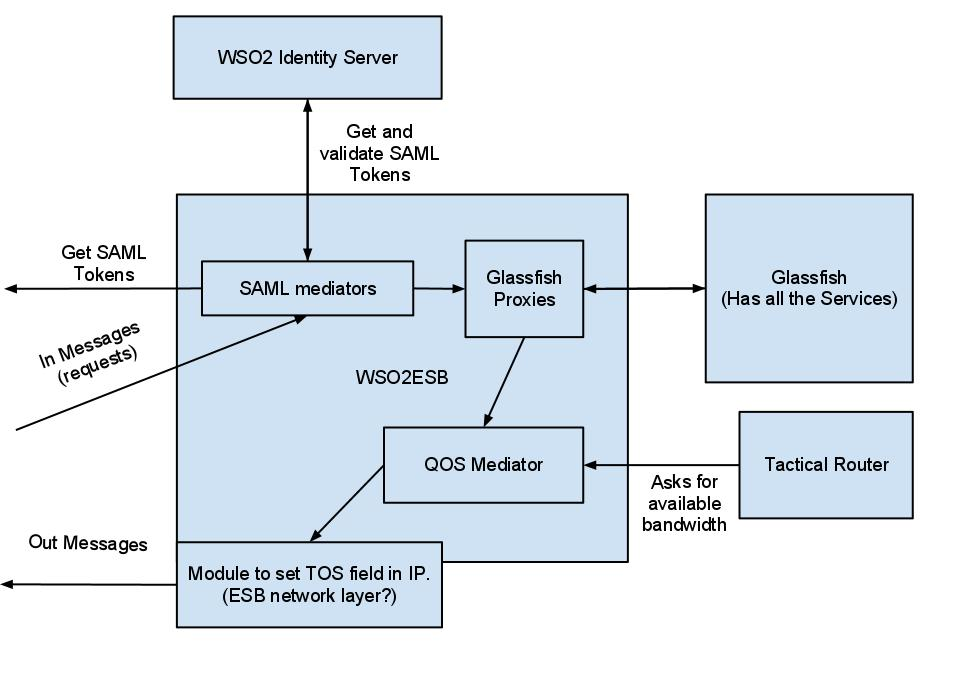
\includegraphics[scale=0.5]{serverside}
            \caption{The serverside architecture}
            \label{fig:serverside}
        \end{figure}

        When the request is received at the service, it will probably start sending some data to the client. This is also done through the ESB. First the message is sent to the QoS mediator. This mediator will first look at the role, or identity, of the client and the service requested, and use this information to assign a priority to the connection. Then the Tactical Router is contacted for bandwidth information, which is used together with the priority to determine whether the message should be sent right away or held back until some higher priority message is finished sending.

        Either in the QoS mediator, in the ESB’s network layer, or after that, the Diffserv (ToS) field of the IP header will have to be set before the message is sent to the client. This field is used by the routers in the network to prioritize packet sending. This step is quite important to the whole procedure as this is one of the few requirements the customer has given us, as such this step can not be dropped from the final product.
        
    \subsection{Client side Architecture}\label{clientsidearch}        
        
\section{Implementation}\label{implementation}
\section{Testing}\label{teting}
\section{Results}\label{results}
\section{Conclusion}\label{conclusion}
    \subsection{Future Work}\label{future}
\section{Project Evaluation}\label{evaluation}

\appendix
\section{Techical Glossary}\label{glossary}
    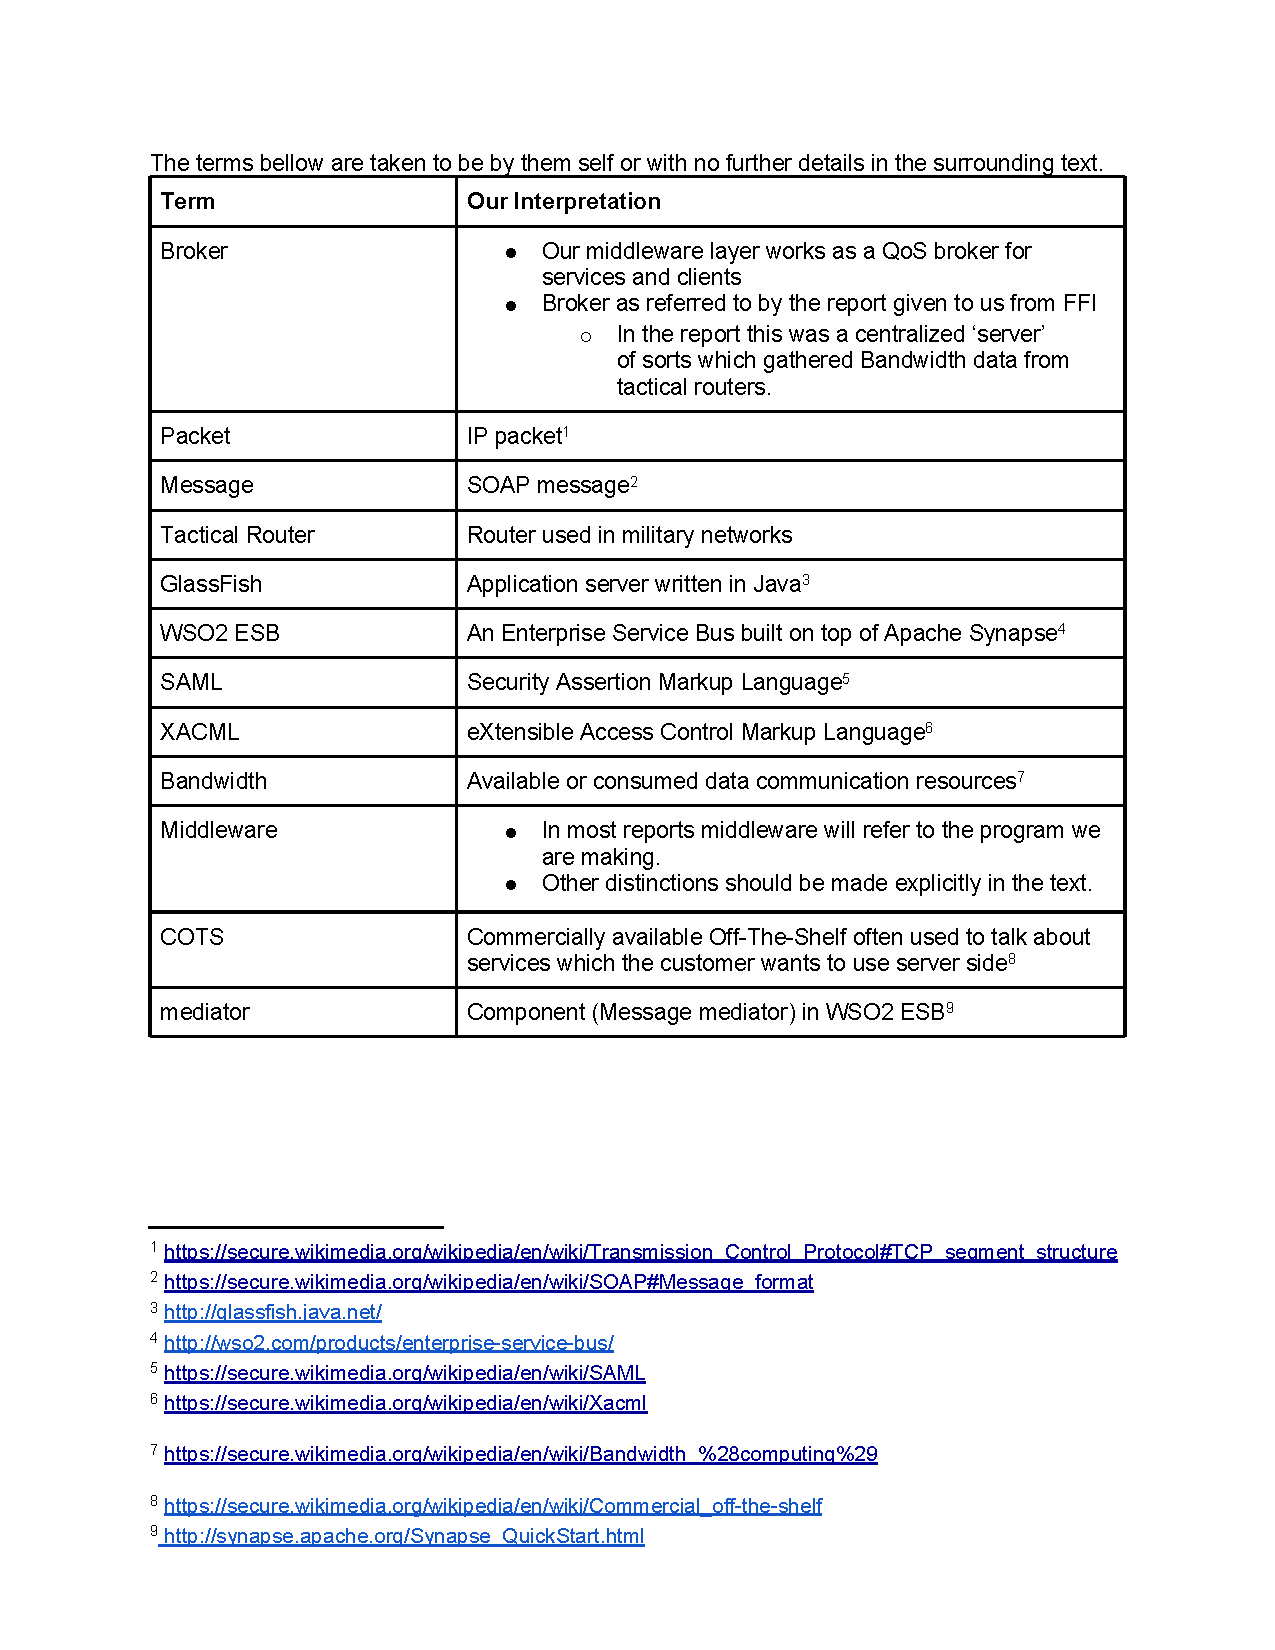
\includepdf{Glossary.pdf}
\section{File Attachments}
    \attachfile[description=TEST log,icon=Paperclip]{report.log} Attached file


\bibliographystyle{abbrv}
\bibliography{main}
\begin{thebibliography}{0}
    \bibitem{lamport94} Leslie Lamport,
        \emph{\LaTeX: A Document Preparation System}.
        Addison Wesley, Massachusetts,
        2nd Edition,
        1994.
    \bibitem{lamport94} 
        Leslie Lamport,
        \emph{\LaTeX: A Document Preparation System}.
        Addison Wesley, Massachusetts,
        2nd Edition,
        1994.
\end{thebibliography}

\end{document}
